\documentclass{sig-alternate}
%\documentclass{acm_proc_article-sp}

\makeatletter
\newif\if@restonecol

\let\algorithm\relax
\let\endalgorithm\relax
\usepackage[tight,footnotesize]{subfigure}
\usepackage {paralist}
\usepackage{comment}
\usepackage{array}
\usepackage{amsmath}
\usepackage{graphicx}
\usepackage{amssymb}
\usepackage{cite}
\usepackage{url}
\makeatother
\makeatletter
\providecommand{\tabularnewline}{\\}


\newtheorem{clm}{Claim}
\begin{document}

\title{STM Concurrency Control for Multicore Embedded Real-Time Software: Time Bounds and Tradeoffs%\thanks{\footnotesize{Approved for Public Release. Unlimited Distribution.}}
}


\author{}
%\alignauthor
%Mohammed El-Shambakey\\
%       \affaddr{ECE Dept., Virginia Tech}\\
 %      \affaddr{Blacksburg, VA 24060}\\
%       \affaddr{USA}\\
%       \email{shambake@vt.edu}

%\alignauthor
%Binoy Ravindran\\
% 	\affaddr{ECE Dept., Virginia Tech}\\
 %      \affaddr{Blacksburg, VA 24060}\\
  %     \affaddr{USA}\\
   %    \email{binoy@vt.edu}
%}

\maketitle

\begin{abstract}
We consider software transactional memory (STM) concurrency control in multicore embedded real-time software. We investigate real-time contention managers (CMs) for resolving transactional conflicts, including those based on dynamic and fixed priorities, and establish upper bounds on transactional retries and task response times. We identify the conditions under which STM (with the proposed CMs) is superior to lock-based and lock-free synchronization.

\end{abstract}

\section{Introduction}
\label{sec:intro}

Embedded systems sense physical processes and control their behavior, typically through feedback loops. Since physical processes are concurrent, computations that control them must also be concurrent, enabling them to process multiple streams of sensor input and control multiple actuators, all concurrently. Often, such computations need to concurrently read/write shared data objects. Typically, they must also process sensor input and react in a timely manner. 

The de facto standard for programming concurrency is the threads abstraction, and the de facto synchronization abstraction is locks. 
Lock-based concurrency control has significant programmability, scalability, and compositionality challenges~\cite{Herlihy:2006:AMP:1146381.1146382}. Transactional memory (TM) is an alternative synchronization model for shared in-memory data objects that promises to alleviate these difficulties.  With TM, programmers write concurrent code using threads, but organize code that read/write shared objects as transactions, which appear to execute atomically. Two transactions conflict if they access the same object and one access is a write. When that happens, a contention manager (or CM)~\cite{Guerraoui:2005:TTT:1073814.1073863} resolves the conflict by aborting one and allowing the other to proceed to commit, yielding (the illusion of) atomicity. Aborted transactions are re-started, often immediately.  In addition to a simple programming model, TM provides performance comparable or superior to highly concurrent fine-grained locking and lock-free approaches~\cite{Saha:2006:MHP:1122971.1123001}, and is composable~\cite{Harris:2005:CMT:1065944.1065952}. Multiprocessor TM has been proposed in hardware, called HTM (e.g.,~\cite{austenmc:tcc:dissertation:2009}), and in software, called STM (e.g.,~\cite{sha95}), with the usual tradeoffs: HTM provides strong atomicity~\cite{austenmc:tcc:dissertation:2009}, has lesser overhead, but needs transactional support in hardware; STM is available on any hardware.


Given STM's programmability, scalability, and compositionality advantages, we consider it for concurrency control in multicore embedded real-time software. Doing so will require bounding transactional  retries, as real-time threads, which subsume transactions, must satisfy time constraints.  Retry bounds in STM are dependent on the CM policy at hand (analogous to the way thread response time bounds are scheduler-dependent). Thus, real-time CM is logical.

Designing a real-time CM is straightforward. Transactional contention can be resolved using dynamic or fixed priorities of parent threads, resulting in Earliest-Deadline-First (EDF) CM or Rate Monotonic Assignment (RMA)-based CM, respectively. But what upper bounds exist for transactional retries and thread response times under such CMs and respective multicore real-time schedulers, global EDF (G-EDF) and global RMA (G-RMA)? How does real-time STM compare against locking and lock-free protocols? i.e., are there upper or lower bounds for transaction lengths below or above which is STM superior to locking/lock-free?

We answer these questions. We consider EDF and RMA CMs, and establish their retry and response time upper bounds, and the conditions under which they outperform locking and lock-free protocols. Our work reveals a key result: for most cases, for G-EDF/EDF CM and G-RMA/RMA CM to be better or as good as lock-free, the atomic section length under STM must not exceed half of the lock-free retry loop-length. However, in some cases, for G-EDF/EDF CM, the atomic section length can reach the lock-free retry loop-length, and for G-RMA/RMA CM, it can even be larger than the lock-free retry loop-length.  This means that, STM is more advantageous with G-RMA than with G-EDF.
These results, among others, for the first time, provide a
fundamental understanding of when to use, and not use, STM concurrency
control in multicore embedded real-time software, and constitute the
paper's contribution. 

We overview past and related efforts in Section~\ref{sec:past}. Section~\ref{sec:model} outlines the work's preliminaries. Sections~\ref{sec:g-edf-edf-cm} and~\ref{sec:g-rma-rma-cm}
establish response time bounds under G-EDF/EDF CM and G-RMA/RMA CM, 
respectively. We consider the FMLP~\cite{key-4} and OMLP~\cite{key-3} protocols as the best locking competitors to STM, given their superiority, and bound their blocking times in Section~\ref{sec:blocking-bound-fmlp-omlp}. We compare STM against locking and lock-free approaches in Section~\ref{sec:comparison}. We conclude in Section~\ref{sec:conclusions}.

\section{Related Work}
\label{sec:past}

Transactional-like concurrency control without using locks, for real-time systems, has been previously studied in the context of non-blocking data structures (e.g.,~\cite{anderson95realtime}). Despite their numerous advantages over locks 
(e.g., deadlock-freedom), 
their programmability has remained a challenge. 
Past studies show that they are best suited for simple data structures where their retry cost is competitive to the cost of lock-based synchronization~\cite{bc+08}.  In contrast, STM is semantically simpler~\cite{Herlihy:2006:AMP:1146381.1146382}, and is often the only viable lock-free solution for complex data structures (e.g., red/black tree)~\cite{key-1} and nested critical sections~\cite{Saha:2006:MHP:1122971.1123001}. (The relationship between lock-free and STM is similar to that between programmer-controlled memory management and garbage collection.)


STM concurrency control for real-time systems has been previously studied in~\cite{manson2006preemptible,fahmy2009bounding,sarni2009real,schoeberl2010rttm,key-1,barrosmanaging}.


\cite{manson2006preemptible} proposes a restricted version of STM for uniprocessors. Uniprocessors do not need contention management.

\cite{fahmy2009bounding} bounds response times in distributed multiprocessor systems with STM synchronization. They consider Pfair scheduling, limit to small atomic regions with fixed size, and limit transaction execution to span at most two quanta. In contrast, we allow atomic regions with  arbitrary duration. 

\cite{sarni2009real} presents real-time scheduling of transactions and serializes transactions based on deadlines. However, the work does not bound retries and response times, nor establishes  tradeoffs against locking and lock-free approaches. In contrast, we establish such bounds and tradeoffs.


\cite{schoeberl2010rttm} proposes real-time HTM, unlike real-time STM that we consider. 
The work does not describe how transactional conflicts are resolved. 
In contrast, we show how task response times can be met using different conflict resolution policies. 
Besides, the retry bound developed in~\cite{schoeberl2010rttm} assumes that the worst case conflict between atomic sections of different tasks occurs when the sections are released at the same time. However, we show that this is not the worst case. We develop retry and response time upper bounds based on much worse conditions.


The past work that is closest to ours is~\cite{key-1}, which upper bounds retries and response times for  EDF CM with G-EDF, and identify the tradeoffs against locking and lock-free protocols. Similar to~\cite{schoeberl2010rttm},~\cite{key-1} also assumes that the worst case conflict between atomic sections occurs when the sections are released simultaneously. 
In addition, we consider RMA CM, besides EDF CM.

The ideas in~\cite{key-1} are extended in~\cite{barrosmanaging}, which presents three real time CM designs. But no retry bounds nor schedulability analysis techniques are presented for those CMs. 


\section{Preliminaries}
\label{sec:model}

We consider a multiprocessor system with $m$ identical processors and $n$ sporadic tasks $T_1, T_2,\ldots, T_n$. The $k^{th}$ instance (or job) of a task $T_i$ is denoted $T_i^k$. Each task $T_i$ is specified by its worst case execution time (WCET) $c_i$, its minimum period $t(T_i)$ between any two consecutive instances, and its relative deadline $D(T_i)$, where $D(T_i)=t(T_i)$. Job $T_i^j$ is released at time $r(T_i^j)$ and must finish no later than its absolute deadline $d(T_i^j)=r(T_i^j)+D(T_i)$. Under a fixed priority scheduler such as G-RMA, $p(T_i)$ determines $T_i$'s (fixed) priority. Under a dynamic priority scheduler such as G-EDF, a job's priority is determined by its absolute deadline. 
A task $T_j$ may interfere with task $T_i$ for a number of times during a duration $L$, and this number is denoted as $G_{ij}(L)$. 
$T_j$'s workload that interferes with $T_i$ during $L$ is denoted $W_{ij}(L)$.


\textit{Shared objects.} A task may need to access (i.e., read, write) shared, in-memory objects while it is executing any of its atomic sections, which are synchronized using STM. 
The set of atomic sections of task $T_i$ is denoted $s_i$. $s_i^k$ is the $k^{th}$ atomic section of $T_i$. 
Each object, $\theta$, can be accessed by multiple tasks. The set of objects accessed by $T_i$ is $\theta_i$.
The set of atomic sections used by $T_i$ to access $\theta$ is $s_i(\theta)$, and the sum of the lengths of those atomic sections is $len(s_i(\theta))$. 

$s_i^k(\theta)$ is the $k^{th}$ atomic section of $T_i$ that accesses $\theta$. $s_i^k(\theta)$  executes for a duration $len(s_i^k(\theta))$, which is the whole length of the atomic section (and not just the part that accesses $\theta$). 
Thus, for two objects $\theta_1$ and $\theta_2$ that are accessed within the same atomic section of $T_i$, $len(s_i^k(\theta1))=len(s_i^k(\theta2))$. 
If $\theta$ is shared by multiple tasks, then $s(\theta)$ is the set of atomic sections of all tasks accessing $\theta$, and the set of tasks sharing $\theta$ with $T_i$ is denoted $\gamma (\theta)$. Atomic sections are non-nested.

The maximum-length atomic section in $T_i$ that accesses $\theta$ is denoted $s_{i_{max}} (\theta)$, while the maximum one among all tasks is $s_{max} (\theta)$, and the maximum one among tasks with priorities lower than or equal to that of $T_i$ is $s_{max}^i (\theta)$.

\textit{STM retry cost.} If two or more atomic sections conflict, the CM will commit one section and abort and retry the others, increasing the time to execute the aborted sections. The increased time that an atomic section $s_i^p (\theta)$ will take to execute due to interference with another section $s_j^k (\theta)$, is denoted $W_{i}^{p}(s_{j}^{k}(\theta))$. 

The total time that a task $T_i$'s atomic sections have to retry is denoted $RC(T_i)$.
When this retry cost is calculated over the task period $t(T_i)$ or an interval $L$, it is   denoted, respectively, as $RC(t(T_i))$ and $RC(L(T_i))$. 

\section{G-EDF/EDF CM Response Time}
\label{sec:g-edf-edf-cm}

Since only one atomic section among many that share the same object can commit at any time under STM, those atomic sections execute in sequential order.  A task $T_{i}$'s atomic sections are interfered by other tasks that share the same objects with $T_{i}$. An atomic section of $T_i$, $s_i^k(\theta)$, is aborted and retried by a conflicting atomic section of $T_j$, $s_j^l(\theta)$, if $d(T_j) \le d(T_i)$, by the EDF CM. We will use \emph{ECM} to refer to a multiprocessor system scheduled by G-EDF and resolves STM conflicts using the EDF CM. 



The maximum number of times a task $T_{j}$ interferes with $T_{i}$ is given in~\cite{key-2} and is shown in Figure~\ref{fig1}. 
Here, the deadline of an instance of $T_{j}$ coincides
with that of $T_{i}$, and $T_{j}^{1}$ is delayed by its maximum
jitter $J_{j}$, which causes all or part of $T_{j}$'s execution to overlap within $T_{i}$'s period $t(T_i)$.

$T_j$'s maximum workload that interferes with $T_i$ in $t(T_{i})$ is:
\begin{eqnarray}
W_{ij}^{*}\left(t\left(T_{i}\right)\right) & = & \left\lfloor\frac{t\left(T_{i}\right)}{t\left(T_{j}\right)}\right\rfloor .c_{j}+min\left(c_{j},t\left(T_{i}\right)-\left\lfloor\frac{t\left(T_{i}\right)}{t\left(T_{j}\right)}\right\rfloor .t\left(T_{j}\right)\right)\nonumber \\
 & \le & \left\lceil\frac{t\left(T_{i}\right)}{t\left(T_{j}\right)}\right\rceil .c_{j}
 \label{eq11}\end{eqnarray}
For an interval $L<t(T_{i})$, the worst case pattern of interference
is shown in Figure~\ref{fig2}, and the workload of $T_{j}$ is:
\begin{equation}
\hat{W}{}_{ij}\left(L\right)=\left(\left\lceil\frac{L-c_{j}}{t\left(T_{j}\right)}\right\rceil+1\right).c_{j}\label{eq12}\end{equation}

Thus, the overall workload, over an interval $R$ is:
\begin{equation}
W_{ij}\left(R\right)=min\left(\hat{W}_{ij}\left(R\right),W_{ij}^{*}\left(t\left(T_{i}\right)\right)\right)\label{eq13}\end{equation}


\begin{figure}%[htbp]
\centering
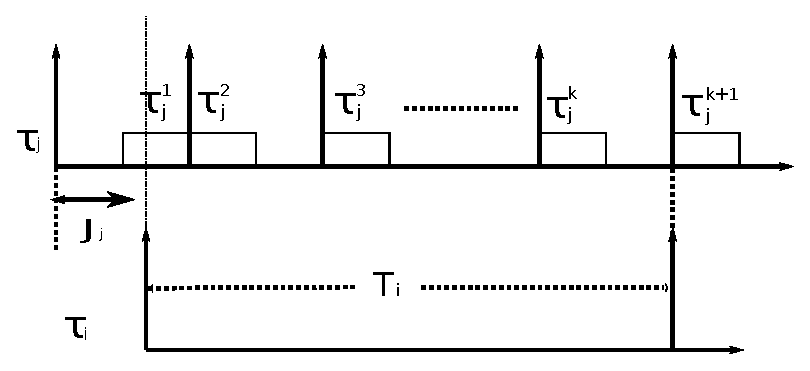
\includegraphics[bb=0bp 0bp 542bp 162bp,scale=0.5]{figures/figure9-a}
\caption{\label{fig1} Maximum interference between two tasks under G-EDF}
\end{figure}


\begin{figure}
\centering
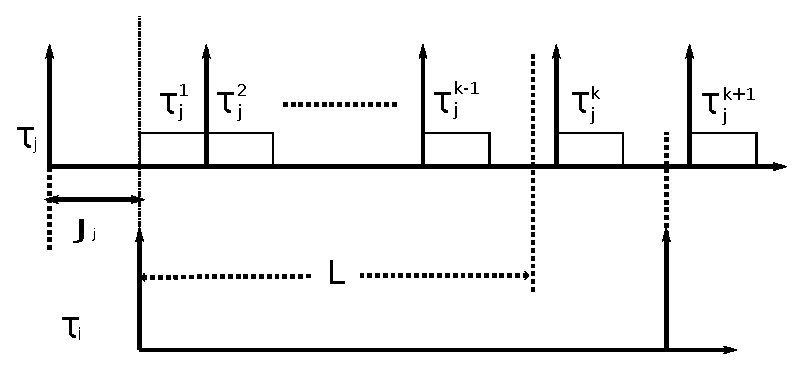
\includegraphics[bb=0bp 0bp 542bp 162bp,scale=0.5]{figures/figure9-b}
\caption{\label{fig2}Maximum interference during part $L$ of $t(T_{i})$}
\end{figure}



\subsection{Retry Cost of Atomic Sections}

\begin{figure*}
\centering
\subfigure[Early validation]{
            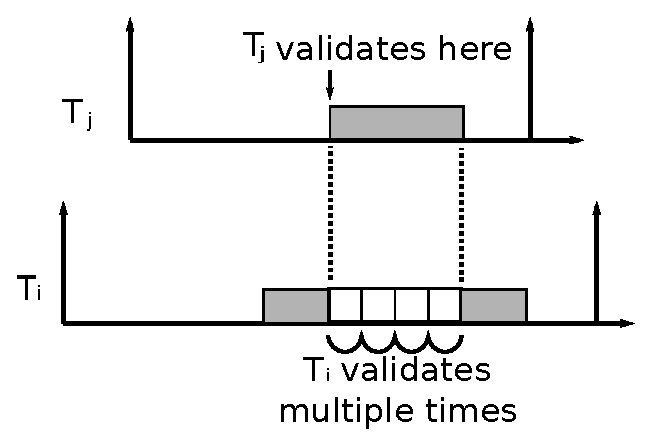
\includegraphics[scale=.45]{figures/figure5-a}
\label{fig5-a} 
}\hspace{1.2cm}
\subfigure[Lazy validation with $s_{i}^{k}(\theta)\le s_{j}^{l}(\theta)$]{
            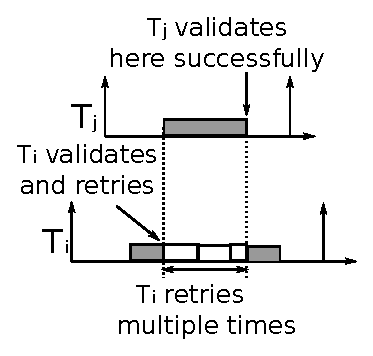
\includegraphics[scale=.65]{figures/figure5-b-1}
\label{fig5-b} 
}\hspace{1.5cm}
\subfigure[Lazy validation with $s_{i}^{k}(\theta)>s_{j}^{l}(\theta)$]{
            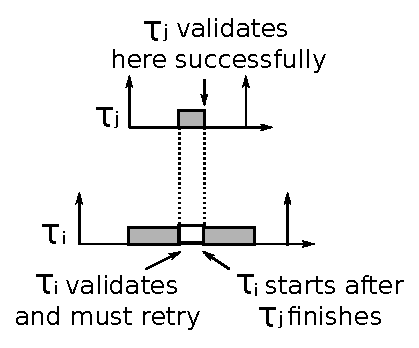
\includegraphics[scale=.65]{figures/figure5-c-1}
\label{fig5-c} 
}
\caption{Retry of $s_i^k(\theta)$ due to $s_j^l(\theta)$}  
\label{fig5}
\end{figure*}

\begin{clm}\label{gedf-edf}
Under ECM, a task $T_i$'s maximum retry cost during $t(T_i)$ is upper bounded by:
\begin{eqnarray}
RC\left(T_{i}\right) & \le & \sum_{\theta\in\theta_{i}}\Big(\Big(\sum_{T_{j}\in\gamma(\theta)}\Big(\left\lceil\frac{t\left(T_{i}\right)}{t\left(T_{j}\right)}\right\rceil\sum_{\forall s_{j}^{l}(\theta)}len\big(s_{j}^{l}(\theta)\nonumber \\
 & + & s_{max}(\theta)\big)\Big)\Big)-s_{max}(\theta)+s_{i_{max}}(\theta)\Big)\label{eq3}\end{eqnarray}
\end{clm}
\begin{proof}
Given two tasks $T_{i}$ and $T_{j}$, where $T_{i}$ has a longer absolute deadline than $T_{j}$. When a shared object conflict occurs, the EDF CM will commit $T_{j}$ and abort and retry $T_{i}$.
Thus, an atomic section of $T_{i}$, $s_{i}^{k}(\theta)$,
will experience its maximum delay when it is at its end of the atomic section, 
%%BR: You can say "...when it is at its end," CORRECT? Since you are referring to the same section. 
and the conflicting atomic section of $T_{j}$, $s_{j}^{l}(\theta)$, starts. 
The CM will retry $s_{i}^{k}(\theta)$. 

Validation (i.e., conflict detection) in STM is usually done in two ways~\cite{austenmc:tcc:dissertation:2009}: a) eager (pessimistic), in which conflicts are detected at access time, b) lazy (optimistic), in which conflicts are detected at commit time. Despite the validation time incurred (either eager or lazy),  
$s_{i}^{k}(\theta)$ will retry for the same time duration, which is $len(s_{j}^{l}(\theta)+s_i^k(\theta))$. Then, $s_i^k(\theta)$ can commit successfully  
unless interferred by another conflicting atomic section, as shown in Figure~\ref{fig5}. 

In Figure~\ref{fig5-a}, $s_{j}^{l}(\theta)$
validates at its beginning, due to early validation, and a conflict
is detected. So $T_{i}$ retries multiple times (because at the start of each retry, $T_{i}$ validates) 
during the execution of $s_{j}^{l}(\theta)$.
When $T_{j}$ finishes its atomic section, $T_{i}$ executes its atomic section. 

In Figure~\ref{fig5-b}, 
$T_{i}$ validates at its end (due to lazy validation), and detects a conflict with $T_{j}$.
Thus, it retries, and because its atomic section length is shorter
than that of $T_{j}$, it validates again within the execution
interval of $s_{j}^{l}(\theta)$. However, the EDF CM retries it again.
This process continues until $T_{j}$ finishes its atomic section.
If $T_{i}$'s atomic section length is longer than that of $T_{j}$'s,
$T_{i}$ would have incurred the same retry time, because
$T_{j}$ will validate when $T_{i}$ is retrying, and $T_{i}$ will
retry again, as shown in Figure~\ref{fig5-c}. Thus, the retry cost
of $s_{i}^{k}(\theta)$ is $len(s_{i}^{k}(\theta)+s_{j}^{l}(\theta))$.

If multiple tasks interfere with $T_{i}$ or
interfere with each other and $T_{i}$ (see the two interference examples in Figure~\ref{fig6}), then, in each case, each atomic section of the shorter deadline tasks contributes to the delay of $s_{i}^{p}(\theta)$ by its total length, plus a retry to some atomic section in the longer deadline tasks. For example,
$s_{j}^{l}(\theta)$ contributes by $len(s_{j}^{l}(\theta)+s_{i}^{p}(\theta))$
in both figures~\ref{fig6-a} and~\ref{fig6-b}. 
%%BR: YOu should say "..in both Figures~\ref{fig6-a} and~\ref{fig6-b}."
In Figure~\ref{fig6-b}, $s_{k}^{y}(\theta)$ causes a retry 
to $s_{j}^{l}(\theta)$, and $s_{h}^{w}(\theta)$ causes a retry to $s_{k}^{y}(\theta)$.


Since we do not know in advance which atomic section will be retried
due to another, we can safely assume that, each atomic section (that share the same object with  $T_i$) in a shorter deadline task contributes by its total length, in addition to the maximum length between all atomic sections that share the same object, $len(s_{max}(\theta))$. Thus, 
\begin{equation}
\mbox{\ensuremath{W_{i}^{p}\left(s_{j}^{k}\left(\theta\right)\right)\le len\left(s_{j}^{k}\left(\theta\right)+s_{max}\left(\theta\right)\right)}}\label{eq2}\end{equation}


Thus, the total contribution of all atomic sections of all other tasks
that share objects with a task $T_i$ 
to the retry cost of $T_i$ during $T_i$'s period $t(T_{i})$ is:
\begin{eqnarray}
RC\left(T_{i}\right) & \le & \sum_{\theta\in\theta_{i}}\sum_{T_{j}\in\gamma(\theta)}\Big(\left\lceil\frac{t\left(T_{i}\right)}{t\left(T_{j}\right)}\right\rceil\sum_{\forall s_{j}^{l}(\theta)}len\big(s_{j}^{l}(\theta)\nonumber \\
 & + & s_{max}(\theta)\big)\Big)\label{eq3-1}\end{eqnarray}



Here, $\left\lceil\frac{t\left(T_{i}\right)}{t\left(T_{j}\right)}\right\rceil\sum_{\forall s_{j}^{l}\left(\theta\right)}len\left(s_{j}^{l}\left(\theta\right)+s_{max}\left(\theta\right)\right)$ is  the contribution of all instances of $T_{j}$ during $t(T_{i})$. This contribution is added to all tasks. The last atomic section to execute is $s_{i}^{p}(\theta)$ ($T_i$'s atomic section that was delayed by conflicting atomic sections of other tasks). One of the other atomic sections (e.g., $s_{m}^{n}(\theta)$) should have a contribution $len(s_{m}^{n}(\theta)+s_{i_{max}}(\theta))$, instead of $len(s_{m}^{n}(\theta)+s_{max}(\theta))$. That is why one $s_{max}(\theta)$ should be subtracted, and $s_{i_{max}}(\theta)$ should be added (i.e., $s_{i_{max}}(\theta)-s_{max}(\theta)$). Claim follows.
\end{proof}

\begin{figure*}%[htbp]%
\centering%
\subfigure[Other atomic sections interfere only with $s_i^p(\theta)$]{
            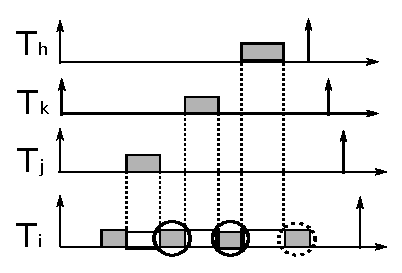
\includegraphics[scale=.65]{figures/figure6-a-1}
\label{fig6-a} 
}\hspace{1cm}
\subfigure[All atomic sections interfere with each other and $s_i^p(\theta)$]{
            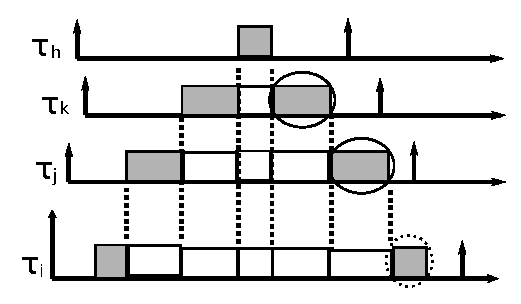
\includegraphics[scale=.6]{figures/figure6-b}
\label{fig6-b} 
}
\begin{tabular}{>{\centering}p{1cm}l}
\includegraphics[scale=0.45]{figures/circle} & Replaced in calculations by $s_{max}(\theta)$\tabularnewline
\includegraphics[scale=0.45]{figures/dotted_circle} & Replaced in calculations by $s_{i_{max}}(\theta)$\tabularnewline
\end{tabular}
\caption{Retry of $s_i^p(\theta)$ due to other atomic sections}  
\label{fig6}
\end{figure*}

\begin{clm}
Claim~\ref{gedf-edf}'s retry bound can be minimized as:
\begin{equation}
RC(T_{i})\le \sum_{\theta\in\theta_{i}}min(\Phi_1 , \Phi_2)\label{eq5}\end{equation}
where $\Phi_1$ is calculated by (\ref{eq3}) for one object $\theta$ (not the sum of $\theta \in \theta_i$),  and 
\begin{eqnarray}
\Phi_2 & = & \Big(\sum_{T_{j}\in\gamma(\theta)} \Big(\left\lceil\frac{t\left(T_{i}\right)}{t\left(T_{j}\right)}\right\rceil\sum_{\forall s_{j}^{l}(\theta)}len \big(s_{j}^{l}(\theta)\nonumber \\
 &  & +s_{max}^{*}(\theta) \big) \Big) \Big)-\bar{s}_{max}(\theta)+s_{i_{max}}(\theta)\label{eq4}\end{eqnarray}
\end{clm}
\begin{proof}
(\ref{eq3}) can be modified by noting that a task $T_i$'s atomic section 
may conflict with those of other tasks, but not with $T_i$. 
This is because, tasks are assumed to arrive sporadically, and  each instance finishes before the next begins. 
Thus, (\ref{eq3}) becomes:
\begin{eqnarray}
RC(T_{i}) & \le & \sum_{\forall\theta\in\theta_{i}} \Big( \Big(\sum_{T_{j}\in\gamma(\theta)} \Big(\left\lceil\frac{t\left(T_{i}\right)}{t\left(T_{j}\right)}\right\rceil\sum_{\forall s_{j}^{l}(\theta)}len \big(s_{j}^{l}(\theta)\nonumber \\
 &  & +s_{max}^{*}(\theta) \big) \Big) \Big)-\bar{s}_{max}(\theta)+s_{i_{max}}(\theta) \Big)\label{eq4-1}\end{eqnarray}
where, $s_{max}^{*}(\theta)\in s(\theta)$ and $s_{max}^{*}(\theta)\not\in s_{j}(\theta)$, 
because $T_{j}$ will not cause a retry to one of its instances.


To obtain $\bar{s}{}_{max}(\theta)$, the maximum-length atomic section of each task that accesses $\theta$ is grouped into an array, in non-increasing order of their lengths. $s_{max}(\theta)$ will be the first element of this array, and $\bar{s}_{max}(\theta)$ will be the next element, as illustrated in Figure~\ref{fig7}, where the maximum atomic
section of each task that accesses $\theta$ is associated with
its corresponding task. In (\ref{eq4-1}), all tasks
but $T_{j}$ will choose $s_{j_{max}}(\theta)$ as the value of $s_{max}^{*}(\theta)$,
as it is the maximum-length atomic section not associated with the interfering task. 
But when $T_{j}$ is the one whose contribution is studied,
it will choose $s_{k_{max}}(\theta)$, as it is the maximum one not
associated with $T_{j}$. This way, it can be seen that the maximum
value always lies between the two values $s_{jmax}(\theta)$ and $s_{kmax}(\theta)$. 
Of course, these two values can be equal, or the maximum value can be associated with $T_i$ itself, and not with any one of the interfering tasks. In the latter case,
the chosen value will always be the one associated with $T_i$, and yet, it will lie between the two largest values. 

\begin{figure}[htbp]
\centering
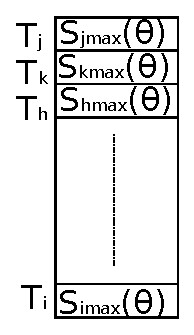
\includegraphics[scale=0.7]{figures/figure7}
\caption{\label{fig7}Values associated with $s_{max}^{*}(\theta)$}
\end{figure}


This means that the subtracted $s_{max}(\theta)$ in (\ref{eq3})
must be replaced with one of these two values ($s_{max}(\theta)$ or $\bar{s}_{max}(\theta)$). However, since we do not know  which task will interfere with $T_i$, the minimum is chosen, as we are determining the worst case retry cost (as this value is going to be subtracted),
and this minimum is the second maximum.


Let $p_j = \left\lceil{\frac{t(T_{i})}{t(T_{j})}}\right\rceil$,
$g_j$ be the number of times $T_j$ accesses $\theta$,  
and 
$Const_j = \left\lceil{\frac{t(T_{i})}{t(T_{j})}}\right\rceil \times \sum_{\forall{s_{j}^{l}(\theta)}}{len(s_{j}^{l}(\theta))}$. 
If $\theta_1$'s maximum-length atomic section is associated with $T_i$ (i.e., $s_{max}(\theta_1)=s_{i_{max}}(\theta_1)$), all other tasks will choose it, and $\Phi_1$ (the result of (\ref{eq3}) for $\theta_1$) will be 
$\sum_{\forall {T_j \in \gamma(\theta_1)}} \left(Const_j +p_j g_j s_{i_{max}}(\theta_1)\right)-s_{i_{max}}(\theta_1)+s_{i_{max}}(\theta_1)$,
whereas $\Phi_2$ (the result of (\ref{eq4-1}) for $\theta_1$) will be $\sum_{\forall {T_j \in \gamma(\theta_1)}} \left(Const_j+ p_j g_j s_{i_{max}}(\theta_1)\right)-s_{k_{max}}(\theta_1)+s_{i_{max}}(\theta_1)$. 
Since $s_{k_{max}}(\theta_1)\leq s_{i_{max}}(\theta_1)$, $\Phi_1 \le \Phi_2$.


Let the maximum-length atomic section for $\theta_2$ be $s_{d_{max}}(\theta_2)$  
($s_{max}(\theta_2)=s_{d_{max}}(\theta_2)$), 
and be associated with another task $T_{d}$, and not with $T_{i}$. Let $ s_{k_{max}}(\theta_2) = \bar{s}_{max}(\theta_2)$,  which will be the second minimum. 
Let $T_{d}$ has $g_d$ atomic sections that share $\theta_2$ with $T_i$. Then, $\Phi_1$ 
for $\theta_2$ will result in $\sum_{\forall T_j \in \gamma(\theta_2)} \left(Const_j +p_j g_j s_{d_{max}}(\theta_2)\right) -s_{d_{max}}(\theta_2)+s_{i_{max}}(\theta_2)$,
and $\Phi_2$ will be $\sum_{\forall T_j \in \gamma(\theta_2) \wedge T_j \ne T_d} \left(Const_j+ p_j g_j s_{d_{max}}(\theta_2)\right)+ Const_d+p_d g_d s_{k_{max}}(\theta_2) -s_{k_{max}}(\theta_2)+s_{i_{max}}(\theta_2)$. So, $\Phi_1 - \Phi_2 =(p_d g_d -1)(s_{d_{max}}(\theta_2)-s_{k_{max}}(\theta_2))$. Since $T_d$ has at least one job that shares $\theta_2$ with $T_i$ (otherwise, $T_d$ would not be included in $\gamma (\theta_2)$), $p_d g_d -1 \ge 0$. Since $s_{d_{max}}(\theta_2) \ge s_{k_{max}}(\theta_2)$, $\Phi_1 \ge \Phi_2$. 


Thus, given an object $\theta$, $\Phi_1$ may be greater, smaller, or equal to $\Phi_2$. The minimum of $\Phi_1$ and $\Phi_2$ therefore yields the worst-case contribution for $\theta$ in $RC(T_i)$. Claim follows.
\end{proof}


\subsection{Upper Bound on Response Time}

To obtain an upper bound on the response time of a task $T_{i}$, the term $RC(T_{i})$ must be added to the workload of other tasks during the non-atomic
execution of $T_{i}$. But this requires modification of the WCET of each
task as follows. 
%starthere
The WCET, $c_{j}$, of each interfering task $T_{j}$ should be inflated to accommodate for the interference of tasks other than $T_{k},$ $k\ne j,i$. Meanwhile, atomic regions that access shared objects between $T_{j}$ and $T_{i}$ should not be considered in the inflation cost, because they have already been calculated in $T_{i}$'s retry cost. Thus, $T_{j}$'s inflated WCET becomes:
\begin{equation}
c_{ji}=c_{j}-\left(\sum_{\theta\in(\theta_{j}\wedge\theta_{i})}len \left(s_{j}(\theta) \right) \right)+RC(T_{ji})\label{eq9}\end{equation}
where, $c_{ji}$ is the new WCET of $T_{j}$ relative to $T_{i}$; 
the sum of lengths of all atomic sections in $T_{j}$ that access object $\theta$ is $\sum_{\theta \in (\theta_j \wedge \theta_i)} {len(s_{j}(\theta))}$; and $RC(T_{ji})$ is the $RC(T_j)$ 
 without including the shared objects between $T_{i}$ and $T_{j}$.
The calculated WCET is relative to task $T_{i}$, as it changes from task to task. The upper bound on the response time of $T_{i}$, denoted $R_{i}^{up}$, can be calculated iteratively, using a modification of Theorem 6 in~\cite{key-2}, as follows:
\begin{equation}
R_{i}^{up}=c_{i}+RC(T_{i})+\left\lfloor\frac{1}{m}\sum_{j\ne i}W_{ij}(R_{i}^{up})\right\rfloor
\label{eq10}
\end{equation}
where $R_{i}^{up}$'s initial value is $c_{i}+RC(T_{i})$.

$W_{ij}(R_{i}^{up})$ is calculated by (\ref{eq13}), and $W_{ij}^{*}(t(T_{i}))$
is calculated by (\ref{eq11}), with $c_{j}$ replaced by 
$c_{ji}$, and changing $\hat{W}_{ij}(L)$ as:
\begin{equation}
\hat{W}_{ij}(L(T_{i}))=max\begin{cases}
\left(\left\lceil\frac{L-c_{ji}-\sum_{\theta\in(\theta_{j}\wedge\theta_{i})}len(s_{j}(\theta))}{t(T_{j})}\right\rceil+1 \right).c_{ji}\\
\left\lceil\frac{L-c_{j}}{t(T_{j})}\right\rceil.c_{ji}+c_{j}-\sum_{\theta\in(\theta_{j}\wedge\theta_{i})}len(s_{j}(\theta))\end{cases}\label{eq14}\end{equation}

(\ref{eq14}) compares between two terms, as we have two cases:


\textit{Case 1}. The carried-in job (i.e., a job whose release is before $r(T_i)$ and its deadline is after $r(T_i)$ but before $d(T_i)$, as defined in~\cite{key-2}) of $T_j$
contributes by $c_{ji}$. Thus, other instances of $T_j$ will begin after this modified WCET, but the sum of the shared objects' atomic section lengths is removed from $c_{ji}$, causing other instances to start earlier. Thus, the term $\sum_{\theta\in(\theta_i\wedge\theta_j)} {len(s_{j}(\theta))}$ is added to $c_{ji}$ to obtain the correct start time. 

\textit{Case 2}. $T_j$'s carried-in job contributes its $c_j$. Thus, other instances begin after this $c_j$ of the carried-in job (as shown in Figure~\ref{fig2}), but the sum of the shared atomic section lengths  between $T_i$ and $T_j$ should be subtracted from this carried-in
instance, as they are already included in the retry cost. 

It should be noted that subtraction of the sum of the shared objects' atomic section lengths is done in the first case to obtain the correct start time of other instances, while in the second case, this is done to get the correct contribution of the carried-in  instance. The maximum is chosen from the two terms in (\ref{eq14}), because they differ in the contribution of their carried-in jobs, and the number of instances after that.

\subsubsection{Tighter Upper Bound}

To tighten $T_{i}$'s response time upper bound, the response time can be calculated recursively over duration $R_i^{up}$, 
and not directly over $t(T_i)$, as done in (\ref{eq10}). Thus, $RC(T_{i})$ will change according
to $T_i$'s recursive response time (i.e., $R_{i}^{up}$). So, (\ref{eq5}) must be changed to include the modified number of interfering instances, in the same way this term  
is calculated in (\ref{eq13}). Also, when calculating this term 
for the entire $t(T_{i})$, a situation like that shown in Figure
\ref{fig10} can happen.
\begin{figure}
\centering{}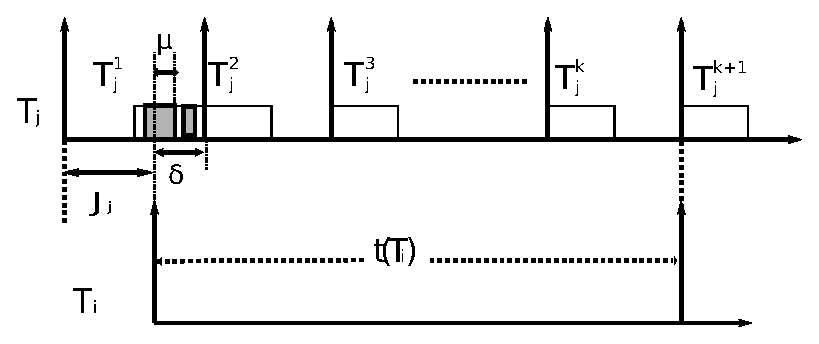
\includegraphics[scale=0.5]{figures/figure10}\caption{\label{fig10} Atomic sections of job $T_{j}^{1}$ contributing to period $t(T_i)$}
\end{figure}


Atomic sections of $T_{j}^{1}$ that are contained in the interval $\delta$
are the only ones that can contribute to $RC(T_{i})$. Of course, they can be lower, but cannot be greater, because $T_{j}^{1}$ has been delayed by its maximum jitter. Hence, no more atomic sections
can interfere during the duration 
$[d(T_{j}^{1})-\delta,d(T_{j}^{1})]$. Even though only one of $T_j^1$'s atomic sections contributes by length $\mu$ to $T_i$, the effect of this $\mu$ will still be the retry of one of the other atomic sections. 

For simplicity, we use the following notations:
\begin{compactitem}
\item $\lambda_{1}\left(j,\theta\right)=\sum_{\forall s_{j}^{l}\left(\theta\right)\in\left[d\left(T_{j}^{1}\right)-\delta,d\left(T_{j}^{1}\right)\right]^{*}}len\left(s_{j}^{l^{*}}\left(\theta\right)+s_{max}\left(\theta\right)\right)$
\item $\chi_{1}\left(i,j,\theta\right)=\left\lfloor\frac{t\left(T_{i}\right)}{t\left(T_{j}\right)}\right\rfloor\sum_{\forall s_{j}^{l}\left(\theta\right)}len\left(s_{j}^{l}\left(\theta\right)+s_{max}\left(\theta\right)\right)$
\item $\lambda_{2}\left(j,\theta\right)=\sum_{\forall s_{j}^{l}\left(\theta\right)\in\left[d\left(T_{j}^{1}\right)-\delta,d\left(T_{j}^{1}\right)\right]^{*}}len\left(s_{j}^{l^{*}}\left(\theta\right)+s_{max}^{*}\left(\theta\right)\right)$
\item $\chi_{2}\left(i,j,\theta\right)=\left\lceil\frac{t\left(T_{i}\right)}{t\left(T_{j}\right)}\right\rceil\sum_{\forall s_{j}^{l}\left(\theta\right)}len\left(s_{j}^{l}\left(\theta\right)+s_{max}^{*}\left(\theta\right)\right)$
\end{compactitem}
Here, $s_{j}^{l^{*}}\left(\theta\right)$ is the part of $s_{j}^{l}\left(\theta\right)$ that
is included in interval $\delta$. The term $\left[d\left(T_{j}^{1}\right)-\delta,d\left(T_{j}^{1}\right)\right]^{*}$ contains $s_{j}^{l}\left(\theta\right)$, whether it is partially or totally included in it. If it is partially included, $s_{j}^{l}(\theta)$
will contribute by its included length $\mu$.

Now, (\ref{eq5}) can be modified as:
\begin{equation}
RC_{}\left(t\left(T_{i}\right)\right)\le \sum_{\theta\in\theta_{i}}min\begin{cases}
\begin{cases}
\Bigl(\left(\sum_{T_{j}\in\gamma\left(\theta\right)}\lambda_{1}\left(j,\theta\right)+\chi_{1}\left(i,j,\theta\right)\right)\\
-s_{max}\left(\theta\right)+s_{i_{max}}\left(\theta\right)\Bigr)\end{cases}\\
\begin{cases}
\Bigl(\left(\sum_{T_{j}\in\gamma\left(\theta\right)}\lambda_{2}\left(j,\theta\right)+\chi_{2}\left(i,j,\theta\right)\right)\\
-\bar{s}_{max}\left(\theta\right)+s_{i_{max}}\left(\theta\right)\Bigr)\end{cases}\end{cases}\label{eq15}\end{equation}



We can compute $RC\left(T_{i}\right)$ during a duration of length $L$, which does not extend to the last instance of $T_{j}$. Let:
\begin{compactitem}
\item $\upsilon\left(L,j\right)=\left\lceil\frac{L-c_{j}}{t\left(T_{j}\right)}\right\rceil+1$
\item $\lambda_{3}\left(j,\theta\right)=\sum_{\forall s_{j}^{l}\left(\theta\right)}len\left(s_{j}^{l}\left(\theta\right)+s_{max}\left(\theta\right)\right)$
\item $\lambda_{4}\left(j,\theta\right)=\sum_{\forall s_{j}^{l}\left(\theta\right)}len\left(s_{j}^{l}\left(\theta\right)+s_{max}^{*}\left(\theta\right)\right)$
\end{compactitem}
Now, (\ref{eq5}) becomes: 
\begin{equation}
RC\left(L\left(T_{i}\right)\right)\le \sum_{\theta\in\theta_{i}}min\begin{cases}
\begin{cases}
\left(\sum_{T_{j}\in\gamma\left(\theta\right)}\left(\upsilon\left(L,j\right)\lambda_{3}\left(j,\theta\right)\right)\right)\\
-s_{max}\left(\theta\right)+s_{i_{max}}\left(\theta\right)\end{cases}\\
\begin{cases}
\left(\sum_{T_{j}\in\gamma\left(\theta\right)}\left(\upsilon\left(L,j\right)\lambda_{4}\left(j,\theta\right)\right)\right)\\
-\bar{s}_{max}\left(\theta\right)+s_{i_{max}}\left(\theta\right)\end{cases}\end{cases}\label{eq16}\end{equation}


Thus, an upper bound on $RC(T_i)$ is given by:
\begin{equation}
RC(R_{i}^{up})\le min\begin{cases}
RC(R_{i}^{up}(T_{i}))\\
RC(t(T_{i}))\end{cases}
\label{eq17}
\end{equation}

The final upper bound on $T_{i}$'s response time can be calculated
as in (\ref{eq10}) by replacing $RC(T_{i})$ with
$RC(R_{i}^{up})$.


\section{Conclusions}
\label{sec:conclusions}

Under both ECM and RCM,  
%%BRL: "..both ECM and RCM,..." 
a task incurs $2.s_{max}$ retry cost for each of its atomic section due to a conflict with another task's atomic section. Retries under RCM and lock-free are affected by a larger number of conflicting task instances than under ECM. While task retries under ECM and lock-free are affected by all other tasks, retries under RCM are affected only by higher priority tasks. 
%%BR: Say ECM and RCM in the above paragraph, instead of EDF CM and RMA CM.


STM and lock-free have similar parameters that affect their retry costs---i.e., the number of conflicting jobs and how many times they access shared objects with a task $T_i$, while FMLP and OMLP are affected by the total number of tasks and the number of requests made by $T_i$. This is because, requests in FMLP and OMLP are arranged in a queue, and the order of the requests in the queue does not change (except for the case of OMLP's priority queue). Thus, STM and lock-free can be compared in terms of parameters affecting their retry costs, while STM and locking protocols can only be compared asymptotically. 
%%BR: Correct?


The $s_{max}/r_{max}$ ratio determines whether STM is better or as good as lock-free.   
For ECM, this ratio cannot exceed 1, and it can be 1/2 for higher number of conflicting tasks. For RCM, for the common case, $s_{max}$ must be 1/2 of $r_{max}$, and in some cases, $s_{max}$ can be larger than $r_{max}$ by many orders of magnitude. For locking protocols, a comparative schedulability of STM to that of FMLP and OMLP depends on the number of tasks and processors.

Thus, no synchronization method fits all applications from a timing standpoint; our results shed light on which method to select under what application conditions. From a programmability standpoint, however, STM is semantically as simple as coarse-grain locks.

Our work has only further scratched the surface of real-time STM. The questions that we ask (see Section~\ref{sec:intro}) are fundamentally analytical in nature, and hence, our results are analytical. However, significant insights can be gained by experimental work on a broad range of embedded software, which is outside our work's scope. For example, what are the typical range of values for the different parameters that affect the retry cost (and hence the response time)? How tight is our retry and response time bounds in practice? Can real-time CMs be designed for other multiprocessor real-time schedulers (e.g., partitioned, semi-partitioned), and those that dynamically improve application timeliness behavior? These are important directions for further work. 


\bibliographystyle{abbrv}
\bibliography{global_bibliography}

\end{document}
